%==============================================================================
% Document header
%==============================================================================
\documentclass[a4paper,11pt]{article}

% Margin setup to use more of the page
\usepackage[top=3cm, bottom=3cm, left=2cm, right=2cm]{geometry}

% Color package
\usepackage[usenames,dvipsnames,table]{xcolor}

% Hyperrefs
\usepackage[
  colorlinks = true,
  linkcolor  = black,
  citecolor  = black,
  urlcolor   = blue,
]{hyperref}

% Longtable
\usepackage{longtable}

% Graphics, multirow
\usepackage{graphicx}
\usepackage{multirow}

% Appendix package
\usepackage[toc,page]{appendix}

% Configure header
\usepackage{fancyhdr}
\setlength{\headheight}{15.2pt}
\pagestyle{fancy}
\fancyhead[L]{\nouppercase{\leftmark}}
\fancyhead[R]{}
\renewcommand{\footrulewidth}{0.4pt}

% Row number command
\newcounter{rownr}
\newcommand{\rownumber}{\stepcounter{rownr}\arabic{rownr}}

% AMS symbols
\usepackage{amssymb}

%==============================================================================
% Start of document
%==============================================================================
\begin{document}

%------------------------------------------------------------------------------
% Title
%------------------------------------------------------------------------------
\begin{titlepage}

\begin{figure}[h]
  \includegraphics[height=3cm]{fig/kth-logo}
\end{figure}

\vspace*{3cm}

%---------------------------------------------------------------
% name
%---------------------------------------------------------------
\noindent{\LARGE \textbf{CUBES Interface Control Document for Bench Test Model}}

\noindent \rule{\textwidth}{.1cm}

\hfill 2016-09-09

\vfill

%---------------------------------------------------------------
% name
%---------------------------------------------------------------
\noindent {\Large \textbf{Theodor-Adrian Stana (KTH Particle and Astroparticle Physics)}}

\noindent \rule{\textwidth}{.05cm}

\end{titlepage}


%------------------------------------------------------------------------------
% Licensing info
%------------------------------------------------------------------------------
\pagebreak

\thispagestyle{empty}

\addcontentsline{toc}{section}{Licensing information}
\section*{Licensing information}

\noindent
This document is licensed under a Creative Commons Attribution-ShareAlike 4.0
International License. If you have not received a copy of the license along with this
work, see \\
\url{http://creativecommons.org/licenses/by-sa/4.0/}

%------------------------------------------------------------------------------
% Revision history
%------------------------------------------------------------------------------
\section*{Revision history}
\addcontentsline{toc}{section}{Revision history}

\centerline
{
  \rowcolors{2}{white}{gray!25}
  \begin{tabular}{l c p{.6\textwidth}}
  \hline
  \multicolumn{1}{c}{\textbf{Date}} & \multicolumn{1}{c}{\textbf{Version}} & \multicolumn{1}{c}{\textbf{Change}} \\
  \hline
  2016-09-09 & 1.0 & First draft \\
  \hline
  \end{tabular}
}

%------------------------------------------------------------------------------
% Table of contents, list of figs, tables
%------------------------------------------------------------------------------
\pagebreak
\pdfbookmark[1]{\contentsname}{toc}
\tableofcontents

\listoffigures
\listoftables

%------------------------------------------------------------------------------
% List of abbreviations
%------------------------------------------------------------------------------
\pagebreak
\section*{List of abbreviations}
\begin{tabular}{l l}

BTM & Bench Test Model \\
CUBES & CUBEsat x-ray explorer using Scintillators \\
GAGG & Gd$_3$Al$_2$Ga$_3$O$_{12}$ (scintillator) \\
ICD & Interface Control Document \\
IO & Input/Output \\
OBC & On-Board Computer \\

\end{tabular}
\addcontentsline{toc}{section}{List of abbreviations}

%==============================================================================
% SEC: Intro
%==============================================================================
\pagebreak
\section{Introduction}
\label{sec:intro}

CUBES (CUBEsat x-ray explorer using Scintillators) is a radiation detection experiment
flying on the MIniature STudent satellite (MIST) mission developed by the Royal
Institute of Technology (KTH) in Stockholm. CUBES is planned to map the radiation
environment in orbit around the Earth using Multi-Pixel Photon Counters (MPPCs) from
Hamamatsu and using GAGG (Gd$_3$Al$_2$Ga$_3$O$_{12}$), BGO and plastic scintillators. 
CUBES is a joint collaboration between KTH and Hiroshima University.

This Interface Control Document (ICD) stems from a Skype meeting on 2016-09-07.
The document details splitting of work between KTH and Hiroshima University for the bench 
test model (BTM) to be supplied by December 2016.

The presentations given during the Skype meeting on 2016-09-07 are an extra reference
for this documentation. They are available online \cite{pres}.

%==============================================================================
% SEC: BTM
%==============================================================================
\section{Bench Test Model}

MIST document M600\_001~\cite{m600_001} details various development models in space 
projects, as well as the model followed during development of the MIST satellite.
Table~\ref{tbl:mist-devel-model} lists the stages in the satellite's development and what 
state an experiment should be in at each stage of development.

Since for the BTM to be delivered by December 2016, CUBES should be in a `breadboard`
state, a proposed solution for developing this BTM is shown in
Figure~\ref{fig:btm-diagram}.

\renewcommand{\arraystretch}{1.5} {

\begin{table}[h]
  \rowcolors{2}{white}{gray!25}
  \caption{\label{tbl:mist-devel-model} MIST development model}
  \centerline {
    \begin{tabular}{p{.3\textwidth} l}
    \hline
	    \multicolumn{1}{c}{\textbf{MIST}} & 
	      \multicolumn{1}{c}{HMU \hspace{5pt} $\longrightarrow$ \hspace{5pt} BTM 
	      $\longrightarrow$ \hspace{5pt} PFM} \\
    \hline
    HMU -- Harness Mock-Up & Experiments as simple models (cardboard, 3D prints) \\
    BTM -- Bench Test Model & Experiments as simulators or breadboards \\
    PFM -- Proto-Flight Model & Experiments in flight standard \\
    \hline
    \end{tabular}
  }
\end{table}

}

\begin{figure}[h]
  \centerline{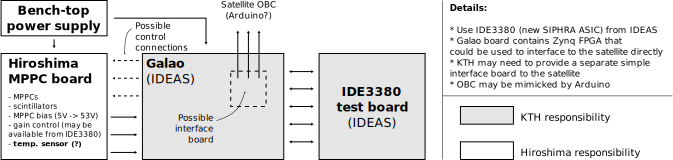
\includegraphics[width=\textwidth]{fig/btm-diagram}}
  \caption{\label{fig:btm-diagram} Bench Test Model diagram}
\end{figure}

\subsection{The Galao development board}

The Galao development board from IDEAS is shown in Figure~\ref{fig:galao}. Its
main features are listed below:

\begin{itemize}
  \item Detector front-end
  \item Connects to separate ASIC development board
  \item Zynq FPGA with IOs accessible
  \item If an ASIC development board is purchased, the Zynq comes with interface
  firmware
\end{itemize}

Since Galao has an FPGA which comes with pre-loaded firmware for interfacing to
ASIC, it is possible that we could add our own VHDL code to interface to the
satellite OBC and thus use it as the core of the BTM.

\begin{figure}[h]
  \centerline{\includegraphics[width=.6\textwidth]{fig/galao.jpg}}
  \caption{\label{fig:galao} The Galao development board}
\end{figure}

%==============================================================================
% SEC: Deliverables
%==============================================================================
\section{Deliverables}

\subsection{KTH}

\begin{itemize}
  \item Galao and IDE3380 development boards
  \item VHDL code for interfacing to the OBC
  \item VHDL code for data structures
  \item Possible board for connecting to Zynq IOs exposed by Galao
  \item Contact with MIST development team
  \item BGO and plastic scintillators (use leftovers from PoGO+)
\end{itemize}

\subsection{Hiroshima}

\begin{itemize}
  \item MPPCs
  \item Bias circuit
  \item GAGG scintillators
  \item Detector light-tightening
\end{itemize}

%==============================================================================
% SEC: Open questions
%==============================================================================
\section{Open questions}

\renewcommand{\labelitemi}{$\square$}

\begin{itemize}
  \item Can the IDE3380 be used with the different light yields of scintillators we use?
  \item What are the vibration requirements?
  \item What type of MPPC do we use - monolithic or array, or a combination of these?
  \item How many MPPCs and scintillators to use? (currently -- 3)
  \item If we decide to use more scintillators, what are the design drivers? Mass?
    Power? Space? Can we do more interesting science with them?
  \item Do we need different biases for different MPPCs?
  \item How do we achieve light-tightness?
  \item What data structure shall we use?
  \item What are the radiation requirements of components on-board?
  \item What are the magnetic dipoles of our components?
  \item Mind the outgassing properties of components
  \item Do we need to cover MPPC assembly with thin layer of material to reduce
  electron background?
\end{itemize}

%==============================================================================
% Bibliography
%==============================================================================
\pagebreak
\bibliographystyle{ieeetr}
\bibliography{btm-icd}
\addcontentsline{toc}{section}{References}

\end{document}
